\section{ Balistic flight over earth:Balistic spherical flight range  angle phi-0 }\label{sec:q3}  
\textit{In this question we consider the ballistic flight over a stationary, spherical Earth (Re = 6,378 km, μ = 398,600 km3/s2).}

  \subsection{Sketch for the geometry}
\begin{figure}[H]
	\centering
	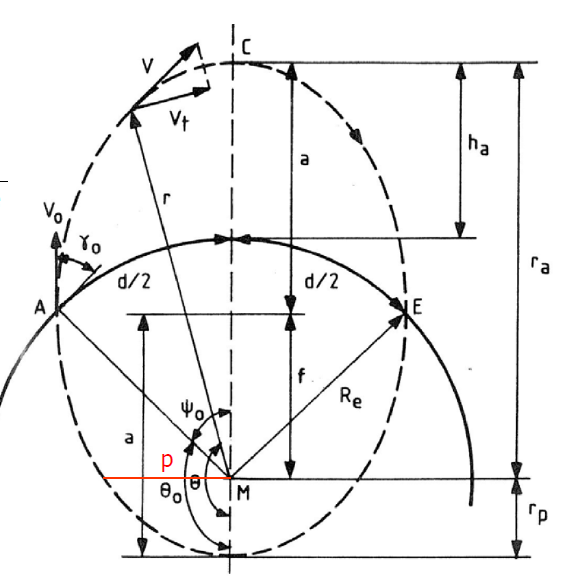
\includegraphics[width=0.4\linewidth]{pics/screenshot001}
	\caption{}
	\label{fig:screenshot001}
\end{figure}

\subsection{Derive the flight-range angle equation}


Derivation in slides 7.8 - 7.16.


Assuming a keplerian trajectory between the shooting point and the final range, and dismissing atmospheric effects, you can apply the vis-viva ecuation in the point A: 

\begin{equation}
\frac{v^2}{2}-\frac{\mu}{r} =\frac{v_0^2}{2}-\frac{\mu}{R_e} =  -\frac{\mu}{2a}
\end{equation}

After some manipulation (see slides for details):
\begin{equation}
\frac{R_ev_0^2}{\mu}-2 = -\frac{R_e}{a}
\end{equation}

Introducing the adimensional velocity (w.r.t.) the velocity of the rotation of the earth:

$$ S_0 = \frac{v_0}{\sqrt{\dfrac{\mu}{R_e}}} $$

The semi-axis is: 

\begin{equation}
\frac{a}{Re} = \frac{1}{2-S_0^2}
\end{equation}

For the semilatus rectum: 
\begin{equation}
\frac{p}{Re} = \frac{H^2}{\mu R_e} = \frac{R_ev_0^2cos^2(\gamma_0)}{\mu} = S_0^2 cos^2(\gamma_0)
\end{equation}

Thus, for the eccentricity, we have:

\begin{equation}
	e=\sqrt{1-\frac{p}{a}} = \sqrt{1-S_0^2 cos^2(\gamma_0)(2-S_0^2)}
\end{equation}

Substituting this into the trajectory equation, we have: 

\begin{equation}
\frac{r}{R_e} = \frac{p/R_e}{1+ e cos(\theta)	} = \frac{ S_0^2 cos^2(\gamma_0)}{1 + \sqrt{1-S_0^2 cos^2(\gamma_0)(2-S_0^2)} cos(\theta)}
\end{equation}

As in the initial point $r = R_e$ and $\theta = \Psi_0 = \frac{d/2}{R_e}$, we can isolate from the previous expression $cos(\Psi_0)$:
\begin{equation}
cos(\Psi_0) = \frac{1 - S_0^2 cos^2(\gamma_0)}{\sqrt{1-S_0^2 cos^2(\gamma_0)(2-S_0^2)} }
\label{ajjaj}
\end{equation}

\subsection{Numerical application}

\textit{For a flight range d = 9,020 km and a launch velocity V0 = 7,905.4 m/s, 	calculate the corresponding launch angle 0.}

First of all, we calculate the adimensional initial velocity parameter $S_0$: 

$$ S_0 = \frac{v_0}{\sqrt{\dfrac{\mu}{R_e}}} =\frac{7,905.4 m/s}{\sqrt{\dfrac{3.986\times 10^{14} m^3/s}{6.278 \times 10^6 m}}} = 1.0000 $$

From Equation \ref{ajjaj}, we obtain that $Psi_0 = 0.7071 rad = 40.51 \degree$.

Substituting $S_0 = 1$ into that Equation, we can isolate the flight path angle:

\begin{align}
cos(\Psi_0) = \frac{1 -  cos^2(\gamma_0)}{\sqrt{1-cos^2(\gamma_0)} } = \sqrt{1-cos^2(\gamma_0)} \\
cos(\gamma_0) = \sqrt{1-cos^2(\Psi_0)} \\
\gamma_0 = 49.4851 \degree
\end{align}